% Options for packages loaded elsewhere
\PassOptionsToPackage{unicode}{hyperref}
\PassOptionsToPackage{hyphens}{url}
\PassOptionsToPackage{dvipsnames,svgnames,x11names}{xcolor}
%
\documentclass[
  letterpaper,
  DIV=11,
  numbers=noendperiod]{scrartcl}

\usepackage{amsmath,amssymb}
\usepackage{iftex}
\ifPDFTeX
  \usepackage[T1]{fontenc}
  \usepackage[utf8]{inputenc}
  \usepackage{textcomp} % provide euro and other symbols
\else % if luatex or xetex
  \usepackage{unicode-math}
  \defaultfontfeatures{Scale=MatchLowercase}
  \defaultfontfeatures[\rmfamily]{Ligatures=TeX,Scale=1}
\fi
\usepackage{lmodern}
\ifPDFTeX\else  
    % xetex/luatex font selection
\fi
% Use upquote if available, for straight quotes in verbatim environments
\IfFileExists{upquote.sty}{\usepackage{upquote}}{}
\IfFileExists{microtype.sty}{% use microtype if available
  \usepackage[]{microtype}
  \UseMicrotypeSet[protrusion]{basicmath} % disable protrusion for tt fonts
}{}
\makeatletter
\@ifundefined{KOMAClassName}{% if non-KOMA class
  \IfFileExists{parskip.sty}{%
    \usepackage{parskip}
  }{% else
    \setlength{\parindent}{0pt}
    \setlength{\parskip}{6pt plus 2pt minus 1pt}}
}{% if KOMA class
  \KOMAoptions{parskip=half}}
\makeatother
\usepackage{xcolor}
\setlength{\emergencystretch}{3em} % prevent overfull lines
\setcounter{secnumdepth}{-\maxdimen} % remove section numbering
% Make \paragraph and \subparagraph free-standing
\makeatletter
\ifx\paragraph\undefined\else
  \let\oldparagraph\paragraph
  \renewcommand{\paragraph}{
    \@ifstar
      \xxxParagraphStar
      \xxxParagraphNoStar
  }
  \newcommand{\xxxParagraphStar}[1]{\oldparagraph*{#1}\mbox{}}
  \newcommand{\xxxParagraphNoStar}[1]{\oldparagraph{#1}\mbox{}}
\fi
\ifx\subparagraph\undefined\else
  \let\oldsubparagraph\subparagraph
  \renewcommand{\subparagraph}{
    \@ifstar
      \xxxSubParagraphStar
      \xxxSubParagraphNoStar
  }
  \newcommand{\xxxSubParagraphStar}[1]{\oldsubparagraph*{#1}\mbox{}}
  \newcommand{\xxxSubParagraphNoStar}[1]{\oldsubparagraph{#1}\mbox{}}
\fi
\makeatother


\providecommand{\tightlist}{%
  \setlength{\itemsep}{0pt}\setlength{\parskip}{0pt}}\usepackage{longtable,booktabs,array}
\usepackage{calc} % for calculating minipage widths
% Correct order of tables after \paragraph or \subparagraph
\usepackage{etoolbox}
\makeatletter
\patchcmd\longtable{\par}{\if@noskipsec\mbox{}\fi\par}{}{}
\makeatother
% Allow footnotes in longtable head/foot
\IfFileExists{footnotehyper.sty}{\usepackage{footnotehyper}}{\usepackage{footnote}}
\makesavenoteenv{longtable}
\usepackage{graphicx}
\makeatletter
\newsavebox\pandoc@box
\newcommand*\pandocbounded[1]{% scales image to fit in text height/width
  \sbox\pandoc@box{#1}%
  \Gscale@div\@tempa{\textheight}{\dimexpr\ht\pandoc@box+\dp\pandoc@box\relax}%
  \Gscale@div\@tempb{\linewidth}{\wd\pandoc@box}%
  \ifdim\@tempb\p@<\@tempa\p@\let\@tempa\@tempb\fi% select the smaller of both
  \ifdim\@tempa\p@<\p@\scalebox{\@tempa}{\usebox\pandoc@box}%
  \else\usebox{\pandoc@box}%
  \fi%
}
% Set default figure placement to htbp
\def\fps@figure{htbp}
\makeatother

\KOMAoption{captions}{tableheading}
\makeatletter
\@ifpackageloaded{tcolorbox}{}{\usepackage[skins,breakable]{tcolorbox}}
\@ifpackageloaded{fontawesome5}{}{\usepackage{fontawesome5}}
\definecolor{quarto-callout-color}{HTML}{909090}
\definecolor{quarto-callout-note-color}{HTML}{0758E5}
\definecolor{quarto-callout-important-color}{HTML}{CC1914}
\definecolor{quarto-callout-warning-color}{HTML}{EB9113}
\definecolor{quarto-callout-tip-color}{HTML}{00A047}
\definecolor{quarto-callout-caution-color}{HTML}{FC5300}
\definecolor{quarto-callout-color-frame}{HTML}{acacac}
\definecolor{quarto-callout-note-color-frame}{HTML}{4582ec}
\definecolor{quarto-callout-important-color-frame}{HTML}{d9534f}
\definecolor{quarto-callout-warning-color-frame}{HTML}{f0ad4e}
\definecolor{quarto-callout-tip-color-frame}{HTML}{02b875}
\definecolor{quarto-callout-caution-color-frame}{HTML}{fd7e14}
\makeatother
\makeatletter
\@ifpackageloaded{caption}{}{\usepackage{caption}}
\AtBeginDocument{%
\ifdefined\contentsname
  \renewcommand*\contentsname{Table of contents}
\else
  \newcommand\contentsname{Table of contents}
\fi
\ifdefined\listfigurename
  \renewcommand*\listfigurename{List of Figures}
\else
  \newcommand\listfigurename{List of Figures}
\fi
\ifdefined\listtablename
  \renewcommand*\listtablename{List of Tables}
\else
  \newcommand\listtablename{List of Tables}
\fi
\ifdefined\figurename
  \renewcommand*\figurename{Figure}
\else
  \newcommand\figurename{Figure}
\fi
\ifdefined\tablename
  \renewcommand*\tablename{Table}
\else
  \newcommand\tablename{Table}
\fi
}
\@ifpackageloaded{float}{}{\usepackage{float}}
\floatstyle{ruled}
\@ifundefined{c@chapter}{\newfloat{codelisting}{h}{lop}}{\newfloat{codelisting}{h}{lop}[chapter]}
\floatname{codelisting}{Listing}
\newcommand*\listoflistings{\listof{codelisting}{List of Listings}}
\makeatother
\makeatletter
\makeatother
\makeatletter
\@ifpackageloaded{caption}{}{\usepackage{caption}}
\@ifpackageloaded{subcaption}{}{\usepackage{subcaption}}
\makeatother

\usepackage{bookmark}

\IfFileExists{xurl.sty}{\usepackage{xurl}}{} % add URL line breaks if available
\urlstyle{same} % disable monospaced font for URLs
\hypersetup{
  pdftitle={Interrogazione di Bagnai alla Camera dei deputati su PMI e Banche},
  pdfauthor={Paolo Volterra},
  colorlinks=true,
  linkcolor={blue},
  filecolor={Maroon},
  citecolor={Blue},
  urlcolor={Blue},
  pdfcreator={LaTeX via pandoc}}


\title{Interrogazione di Bagnai alla Camera dei deputati su PMI e
Banche}
\usepackage{etoolbox}
\makeatletter
\providecommand{\subtitle}[1]{% add subtitle to \maketitle
  \apptocmd{\@title}{\par {\large #1 \par}}{}{}
}
\makeatother
\subtitle{fact checking}
\author{Paolo Volterra}
\date{2025-01-16}

\begin{document}
\maketitle


\pandocbounded{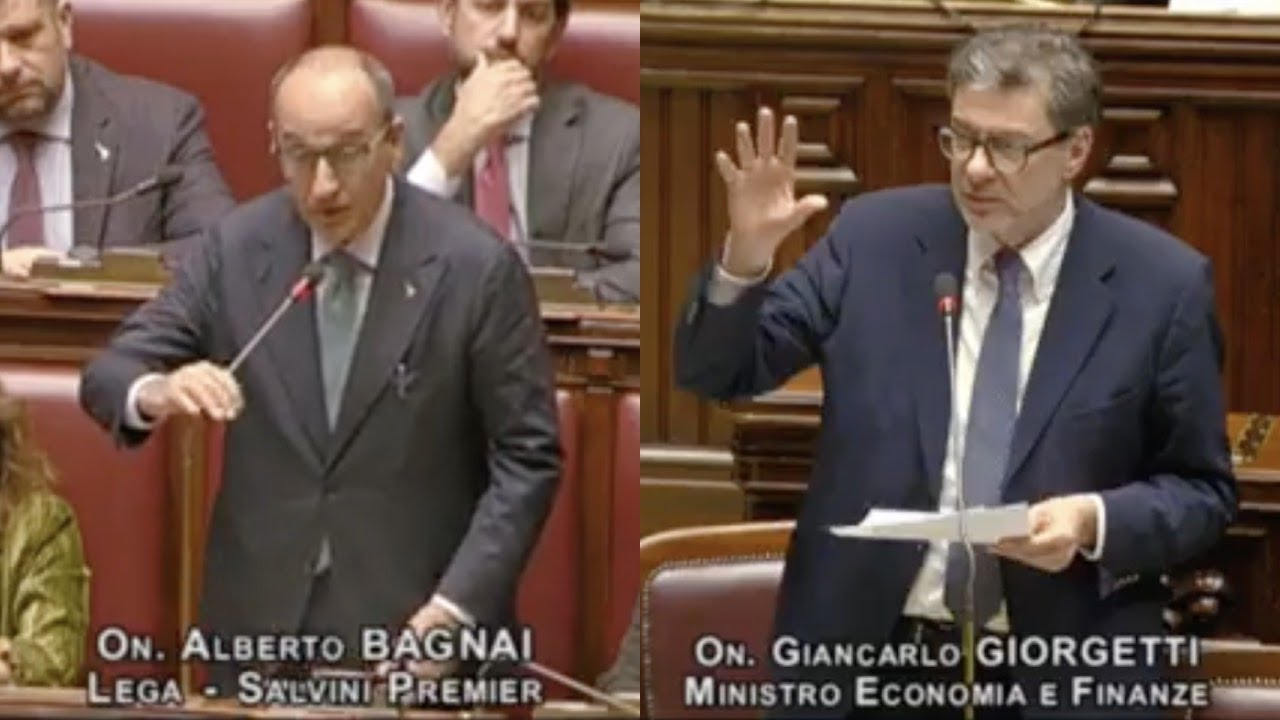
\includegraphics[keepaspectratio]{./media/maxresdefault.jpg}}

costruzione di una pagina di test sui callout e sulle verifiche fatte
con ChatGPT

\section{BAGNAI INTERROGA GIORGETTI SULL'ACCESSO AL CREDITO BANCARIO DA
PARTE DELLE PICCOLE MEDIE
IMPRESE}\label{bagnai-interroga-giorgetti-sullaccesso-al-credito-bancario-da-parte-delle-piccole-medie-imprese}

https://www.youtube.com/watch?v=IUWhHJxyOXw

\subsection{Affermazione 1}\label{affermazione-1}

*``il settore delle piccole e medie imprese è preponderante a livello
europeo in termini numerici. Queste piccole e medie imprese
rappresentano il 99\% in media delle aziende registrate ed esprimono,
sostanzialmente, a livello europeo, i 2/3 degli occupati e circa 1/2 del
valore aggiunto''
(\href{zotero://open-pdf/library/items/B4RMZ7B3?page=1&annotation=4TAI7CT2}{pdf})

\begin{tcolorbox}[enhanced jigsaw, bottomrule=.15mm, opacityback=0, leftrule=.75mm, breakable, titlerule=0mm, left=2mm, title=\textcolor{quarto-callout-warning-color}{\faExclamationTriangle}\hspace{0.5em}{Conclusione}, colframe=quarto-callout-warning-color-frame, coltitle=black, colback=white, toprule=.15mm, colbacktitle=quarto-callout-warning-color!10!white, bottomtitle=1mm, toptitle=1mm, arc=.35mm, rightrule=.15mm, opacitybacktitle=0.6]

La dichiarazione è generalmente corretta.

\end{tcolorbox}

\textbf{Percentuale di PMI sul totale delle imprese:} Le PMI
costituiscono oltre il 99\% di tutte le imprese nell'Unione Europea
(Fonte: Parlamento Europeo, Factsheets on the European Union,
disponibile su
\href{https://www.europarl.europa.eu/factsheets/it/sheet/63/piccole-e-medie-imprese}{europarl.europa.eu}).

\textbf{Occupazione nelle PMI:} Circa due terzi della forza lavoro nel
settore privato è impiegata nelle PMI (Fonte: CORDIS, Observatory of
European SMEs, disponibile su
\href{https://cordis.europa.eu/article/id/18356-observatory-of-european-smes-publishes-first-three-reports}{cordis.europa.eu}).

\textbf{Valore aggiunto generato dalle PMI:} Le PMI contribuiscono a
circa il 56\% del prodotto interno lordo (PIL) dell'UE (Fonte:
Parlamento Europeo, Studio sull'economia europea, disponibile su
\href{https://www.europarl.europa.eu/RegData/etudes/ATAG/2021/690633/EPRS_ATA\%282021\%29690633_IT.pdf}{europarl.europa.eu}).

In sintesi, le PMI rappresentano la spina dorsale dell'economia europea,
con un impatto significativo su occupazione e valore aggiunto.

\begin{center}\rule{0.5\linewidth}{0.5pt}\end{center}

\subsection{Affermazione 2}\label{affermazione-2}

\emph{``a settembre scorso, i primi 10 gruppi bancari per totale
dell'attivo di bilancio detenevano una quota di mercato nazionale di
prestiti alle piccole e medie imprese pari al\%, quindi le prime dieci
banche hanno il 65\% del mercato di prestiti sulle piccole e medie
imprese, con l'eccezione del Trentino-Alto Adige, dove la quota di
mercato dei primi dieci gruppi è minore rispetto alla media nazionale,
sia per i prestiti alle PMI, sia per quelli al complesso delle imprese.
La variabilità delle quote a livello regionale è relativamente
contenuta: si passa dal 48,1\% del Friuli-Venezia Giulia, all'82,5\%
della Sardegna, con percentuali pari al 76,6\% della Liguria, il 70 per
cento della Lombardia e il 59 per cento del Veneto''
(\href{zotero://open-pdf/library/items/B4RMZ7B3?page=1&annotation=T4DLE8D4}{pdf})}

A settembre scorso, i dati confermano che i primi dieci gruppi bancari
in Italia detenevano una quota di mercato nazionale dei prestiti alle
piccole e medie imprese (PMI) pari al \textbf{65\%}. Questo dato è stato
riportato dal ministro dell'Economia Giancarlo Giorgetti durante
un'interrogazione parlamentare{[}1{]}{[}2{]}{[}6{]}.

\subsubsection{Quota di Mercato e Variazioni
Regionali}\label{quota-di-mercato-e-variazioni-regionali}

\begin{itemize}
\tightlist
\item
  \textbf{Quota di Mercato}: Le prime dieci banche, tra cui UniCredit e
  Intesa Sanpaolo, controllano il 65\% del mercato dei prestiti alle
  PMI.
\item
  \textbf{Eccezione del Trentino-Alto Adige}: In questa regione, la
  quota di mercato dei primi dieci gruppi è inferiore rispetto alla
  media nazionale sia per i prestiti alle PMI sia per quelli destinati a
  tutte le imprese{[}1{]}{[}2{]}.
\item
  \textbf{Variabilità Regionale}: Le quote a livello regionale variano
  da un minimo del \textbf{48,1\%} in Friuli-Venezia Giulia a un massimo
  dell'\textbf{82,5\%} in Sardegna. Altre regioni presentano percentuali
  come il \textbf{76,6\%} in Liguria, il \textbf{70,3\%} in Lombardia e
  il \textbf{59,1\%} in Veneto{[}1{]}{[}2{]}{[}6{]}.
\end{itemize}

\subsubsection{Rapporto Prestiti/Attivo}\label{rapporto-prestitiattivo}

Il rapporto tra l'ammontare dei prestiti e il totale attivo di bilancio
per i prestiti alle PMI è mediamente pari al \textbf{9\%}, mentre per il
totale dei prestiti alle imprese è del \textbf{16\%}{[}3{]}{[}4{]}.

\begin{tcolorbox}[enhanced jigsaw, bottomrule=.15mm, opacityback=0, leftrule=.75mm, breakable, titlerule=0mm, left=2mm, title=\textcolor{quarto-callout-warning-color}{\faExclamationTriangle}\hspace{0.5em}{Conclusione}, colframe=quarto-callout-warning-color-frame, coltitle=black, colback=white, toprule=.15mm, colbacktitle=quarto-callout-warning-color!10!white, bottomtitle=1mm, toptitle=1mm, arc=.35mm, rightrule=.15mm, opacitybacktitle=0.6]

In sintesi, l'affermazione riguardo alla quota di mercato delle prime
dieci banche per i prestiti alle PMI è corretta e supportata da dati
ufficiali.

\end{tcolorbox}

\paragraph{Citations:}\label{citations}

\begin{itemize}
\tightlist
\item
  {[}1{]}
  https://www.borsaitaliana.it/borsa/notizie/radiocor/finanza/dettaglio/-
  banche-giorgetti-a-settembre-per-prime-10-rapporto-prestiti-pmiattivi-a-9-nRC\_15012025\_1626\_5196874-
  16.html
\item
  {[}2{]} https://www.ansa.it/sito/notizie/economia/pmi/2025/01/15/-
  giorgetti-prime-10-banche-hanno-65-mercato-prestiti-pmi\_a8fad4c6-414f-46d5-94a1-cdf9d8028aea.html
\item
  {[}3{]} https://www.italiaoggi.it/diritto-e-fisco/diritto-e-impresa/-
  banche-giorgetti-nel-2024-le-imprese-hanno-chiesto-meno-prestiti-hxk4277l
\item
  {[}4{]}
  https://www.confindustria.it/home/centro-studi/prodotti/previsioni/rapporto/highlights/-
  rapporto-previsione-economia-italiana-autunno-2024/4450a521-615e-4af8-b5e0-d2a734796003
\item
  {[}5{]}
  https://www.confindustria.it/home/centro-studi/prodotti/previsioni/rapporto/highlights/-
  rapporto-previsione-economia-italiana-primavera-2024/ca98805a-1f1a-4fef-8d24-1d4e00cfe358
\item
  {[}6{]} https://www.9colonne.it/502477/-
  giorgetti-primi-dieci-gruppi-bancari-a-settembre-scorso-avevano-65-mercato-prestiti-a-pmi
\item
  {[}7{]} https://finanza.lastampa.it/News/2024/11/12/-
  bankitalia-prestiti-ancora-in-calo-a-settembre-per-imprese-2-4percento-su-anno/-
  ODdfMjAyNC0xMS0xMl9UTEI
\item
  {[}8{]}
  https://www.teleborsa.it/News/2024/11/12/bankitalia-prestiti-ancora-in-calo-a-settembre-per-imprese-2-4percent-su-anno-87.html
\end{itemize}

\begin{center}\rule{0.5\linewidth}{0.5pt}\end{center}

\subsection{Affermazione 3}\label{affermazione-3}

\emph{``il rapporto tra l'ammontare dei prestiti e il totale dell'attivo
di bilancio, che ovviamente ricomprende altre voci oltre i prestiti, era
mediamente pari al 9\% nel caso di prestiti alle piccole e medie imprese
e al 16\% con riferimento al complesso dei prestiti alle imprese.
Quindi, dato 100 l'attivo, il 9\% è prestato alle piccole e medie
imprese, il 16\% al complesso. L'andamento dei prestiti alle imprese,
negli scorsi mesi si è andata attenuando la diminuzione dei prestiti
bancari: meno 3,5\% a ottobre, su 12 mesi, cioè continua ma decelera''}

L'affermazione riguardante il rapporto tra l'ammontare dei prestiti e il
totale dell'attivo di bilancio è corretta. I dati confermano che:

\begin{itemize}
\item
  \textbf{Rapporto Prestiti/Attivo}: A settembre, il rapporto tra
  l'ammontare dei prestiti alle piccole e medie imprese (PMI) e il
  totale dell'attivo di bilancio era mediamente pari al \textbf{9\%}.
  Per quanto riguarda il complesso dei prestiti alle imprese, questo
  rapporto era del \textbf{16\%} {[}1{]}{[}4{]}.
\item
  \textbf{Interpretazione dei Dati}: Ciò significa che, su un attivo
  totale di 100, il \textbf{9\%} è prestato alle PMI e il \textbf{16\%}
  al complesso delle imprese.
\item
  \textbf{Andamento dei Prestiti}: Negli ultimi mesi, si è osservata una
  diminuzione dei prestiti bancari, con una contrazione del
  \textbf{3,5\%} a ottobre su base annua. Tuttavia, questa diminuzione
  sta decelerando, indicando una certa stabilizzazione nel mercato del
  credito {[}1{]}{[}4{]}.
\end{itemize}

\begin{tcolorbox}[enhanced jigsaw, bottomrule=.15mm, opacityback=0, leftrule=.75mm, breakable, titlerule=0mm, left=2mm, title=\textcolor{quarto-callout-warning-color}{\faExclamationTriangle}\hspace{0.5em}{Conclusione}, colframe=quarto-callout-warning-color-frame, coltitle=black, colback=white, toprule=.15mm, colbacktitle=quarto-callout-warning-color!10!white, bottomtitle=1mm, toptitle=1mm, arc=.35mm, rightrule=.15mm, opacitybacktitle=0.6]

In sintesi, l'affermazione è supportata da dati ufficiali e riflette
accuratamente la situazione attuale del mercato dei prestiti alle PMI in
Italia.

\end{tcolorbox}

\paragraph{Citations:}\label{citations-1}

\begin{itemize}
\tightlist
\item
  {[}1{]}
  https://www.borsaitaliana.it/borsa/notizie/radiocor/finanza/dettaglio/-
  banche-giorgetti-a-settembre-per-prime-10-rapporto-prestiti-pmiattivi-a-9-nRC\_15012025\_1626\_5196874-
  16.html
\item
  {[}2{]}
  https://www.bancaditalia.it/pubblicazioni/metodi-e-fonti-note/metodi-note-2021/-
  BAM\_note-met\_20211210.pdf
\item
  {[}3{]} https://assets.kpmg.com/content/dam/kpmg/it/pdf/2022/07/-
  KPMG\_AnalisiBilanciGruppiBancariItaliani\_Edizione2022.pdf
\item
  {[}4{]} https://www.ansa.it/sito/notizie/economia/pmi/2025/01/15/-
  giorgetti-prime-10-banche-hanno-65-mercato-prestiti-pmi\_a8fad4c6-414f-46d5-94a1-cdf9d8028aea.html
\item
  {[}5{]}
  https://www.bancaditalia.it/pubblicazioni/conti-finanziari/2025-conti-finanziari/index.html?-
  com.dotmarketing.htmlpage.language=1
\item
  {[}6{]}
  https://docenti.unimc.it/massimo.biasin/teaching/2024/30662/files/kpmg-analisi-bilanci-banche-2024
\end{itemize}

\begin{center}\rule{0.5\linewidth}{0.5pt}\end{center}

\subsection{Affermazione 4}\label{affermazione-4}

\emph{``l'andamento dei prestiti alle imprese, negli scorsi mesi si è
andata attenuando la diminuzione dei prestiti bancari: meno 3,5 per
cento a ottobre, su 12 mesi, cioè continua ma decelera''}

L'affermazione riguardante l'andamento dei prestiti alle imprese è
corretta e supportata da dati recenti. Ecco i punti principali:

\begin{itemize}
\item
  \textbf{Diminuzione dei Prestiti}: A ottobre 2024, i prestiti bancari
  alle imprese hanno registrato una diminuzione del \textbf{3,5\%} su
  base annua. Questo calo è in linea con le tendenze precedenti, ma si
  segnala che la diminuzione sta rallentando rispetto ai tassi più
  elevati di contrazione osservati in passato (ad esempio, un calo del
  \textbf{6,7\%} a settembre 2023) {[}1{]}{[}3{]}.
\item
  \textbf{Decelerazione della Diminuzione}: Il calo dei prestiti è
  ancora presente, ma la sua intensità sta diminuendo. Questo suggerisce
  una stabilizzazione nel mercato del credito, con una possibile ripresa
  in vista {[}1{]}{[}2{]}{[}3{]}.
\item
  \textbf{Richiesta di Credito}: Nonostante la diminuzione dei prestiti,
  la domanda di credito da parte delle imprese continua a essere debole,
  anche se a ritmi più contenuti rispetto ai trimestri precedenti. Ciò è
  attribuibile all'aumento dei tassi di interesse e alla necessità di
  rimborsi su finanziamenti preesistenti {[}1{]}{[}3{]}{[}4{]}.
\end{itemize}

\begin{tcolorbox}[enhanced jigsaw, bottomrule=.15mm, opacityback=0, leftrule=.75mm, breakable, titlerule=0mm, left=2mm, title=\textcolor{quarto-callout-warning-color}{\faExclamationTriangle}\hspace{0.5em}{Conclusione}, colframe=quarto-callout-warning-color-frame, coltitle=black, colback=white, toprule=.15mm, colbacktitle=quarto-callout-warning-color!10!white, bottomtitle=1mm, toptitle=1mm, arc=.35mm, rightrule=.15mm, opacitybacktitle=0.6]

In sintesi, l'affermazione che ``l'andamento dei prestiti alle imprese
negli scorsi mesi si è andata attenuando'' è confermata dai dati
attuali, mostrando una diminuzione del \textbf{3,5\%} a ottobre, con un
trend di decelerazione rispetto ai periodi precedenti.

\end{tcolorbox}

\paragraph{Citations:}\label{citations-2}

\begin{itemize}
\tightlist
\item
  {[}1{]}
  https://www.confindustria.it/home/centro-studi/prodotti/previsioni/rapporto/highlights/-
  rapporto-previsione-economia-italiana-primavera-2024/ca98805a-1f1a-4fef-8d24-1d4e00cfe358
\item
  {[}2{]} https://www.giornaledellepmi.it/-
  report-mensile-abi-a-ottobre-diminuzione-dei-tassi-di-interesse-e-calo-dei-prestiti/
\item
  {[}3{]} https://www.italiaoggi.it/diritto-e-fisco/diritto-e-impresa/-
  banche-giorgetti-nel-2024-le-imprese-hanno-chiesto-meno-prestiti-hxk4277l
\item
  {[}4{]}
  https://www.confindustria.it/home/centro-studi/prodotti/previsioni/rapporto/highlights/-
  rapporto-previsione-economia-italiana-autunno-2024/4450a521-615e-4af8-b5e0-d2a734796003
\item
  {[}5{]}
  https://www.bancaditalia.it/statistiche/tematiche/moneta-intermediari-finanza/-
  intermediari-finanziari/indagine-credito-bancario/risultati/BLS\_Ottobre\_2024.pdf
\item
  {[}6{]} https://www.gaeta.it/-
  diminuzione-tassi-di-interesse-e-calo-prestiti-il-report-mensile-dellabi-per-ottobre-2024
\item
  {[}7{]}
  https://it.marketscreener.com/notizie/ultimo/Banche-Abi-prestiti-in-ripresa-nel-2024-rischiosta-in-aumento-moderato-48131490/
\end{itemize}

\begin{center}\rule{0.5\linewidth}{0.5pt}\end{center}

\subsection{Affermazione 5}\label{affermazione-5}

\emph{``In base all'elaborazione della Banca d'Italia di dati della
Centrale dei rischi Cerved, la flessione dei prestiti è generalizzata
tra classi di rischiosità e dimensione d'impresa''}
(\href{zotero://open-pdf/library/items/B4RMZ7B3?page=2&annotation=33H6DFF3}{pdf})

L'affermazione che ``la flessione dei prestiti è generalizzata tra
classi di rischiosità e dimensione d'impresa'' è supportata dai dati
elaborati dalla Banca d'Italia. Ecco i punti principali:

\begin{itemize}
\item
  \textbf{Flessione Generalizzata}: I prestiti bancari alle imprese
  italiane stanno diminuendo in modo generalizzato, con una contrazione
  che si estende a diverse classi di rischiosità e dimensioni aziendali.
  Questo è confermato dall'indagine della Banca d'Italia, che evidenzia
  come la domanda di credito continui a ridursi, specialmente per i
  prestiti a lungo termine, mentre la diminuzione è meno marcata per
  quelli a breve termine{[}1{]}{[}2{]}.
\item
  \textbf{Dati Recenti}: A febbraio 2024, i prestiti alle imprese hanno
  mostrato una flessione del \textbf{3,8\%} rispetto all'anno
  precedente, sebbene la diminuzione sia meno accentuata rispetto ai
  picchi negativi del 2023, che avevano raggiunto un calo del
  \textbf{6,7\%} a settembre{[}1{]}{[}2{]}.
\item
  \textbf{Impatto delle Condizioni Economiche}: La contrazione dei
  prestiti è influenzata da vari fattori, tra cui l'aumento dei tassi di
  interesse da parte della BCE e le condizioni economiche generali. Le
  imprese manifestano difficoltà nell'accesso al credito, con una
  percentuale significativa che non riesce a ottenere i finanziamenti
  richiesti{[}3{]}{[}4{]}.
\end{itemize}

\begin{tcolorbox}[enhanced jigsaw, bottomrule=.15mm, opacityback=0, leftrule=.75mm, breakable, titlerule=0mm, left=2mm, title=\textcolor{quarto-callout-warning-color}{\faExclamationTriangle}\hspace{0.5em}{Conclusione}, colframe=quarto-callout-warning-color-frame, coltitle=black, colback=white, toprule=.15mm, colbacktitle=quarto-callout-warning-color!10!white, bottomtitle=1mm, toptitle=1mm, arc=.35mm, rightrule=.15mm, opacitybacktitle=0.6]

In sintesi, l'affermazione sulla flessione generalizzata dei prestiti
tra diverse classi di rischiosità e dimensione d'impresa è corretta e
riflette la situazione attuale del mercato del credito in Italia.

\end{tcolorbox}

\paragraph{Citations:}\label{citations-3}

\begin{itemize}
\tightlist
\item
  {[}1{]}
  https://www.confindustria.it/home/centro-studi/prodotti/previsioni/rapporto/highlights/-
  rapporto-previsione-economia-italiana-primavera-2024/ca98805a-1f1a-4fef-8d24-1d4e00cfe358
\item
  {[}2{]}
  https://www.confindustria.it/home/centro-studi/prodotti/previsioni/rapporto/highlights/-
  rapporto-previsione-economia-italiana-autunno-2024/4450a521-615e-4af8-b5e0-d2a734796003
\item
  {[}3{]}
  https://www.bancaditalia.it/statistiche/tematiche/moneta-intermediari-finanza/-
  intermediari-finanziari/indagine-credito-bancario/risultati/BLS\_Luglio\_2024.pdf
\item
  {[}4{]} https://www.simplybiz.eu/-
  banca-ditalia-prestiti-a-famiglie-e-imprese-rapporto-stabilita-finanziaria-2024/
\item
  {[}5{]}
  https://infostat.bancaditalia.it/inquiry/GetDocumentFile?type=PDF\&docId=208675\&-
  cubeId=BAM\_STATICISSUE1
\item
  {[}6{]}
  https://finanza.repubblica.it/News/2024/03/11/bankitalia\_a\_gennaio\_accelera\_il\_calo\_dei\_prestiti\_alle\_imprese-61/
\end{itemize}




\end{document}
